\section{文件共享与PIPE}
文件共享和管道是操作系统中关键的概念,它们为进程之间的通信和协同提供了有效的手段。
在npucore中,这些机制是构建多任务、多进程应用程序的基础。本章将深入探讨文件共享和管道的原理、应用和在npucore中的具体实现。

文件共享是多个进程之间共享数据的一种机制。
我们将深入研究硬链接和软链接,它们分别提供了对同一文件的不同访问方式。

硬链接是文件系统中的重要概念,允许一个文件存在于多个位置,节省存储空间并提供数据的共享。
与硬链接相比,软链接提供了更灵活的方式来共享文件。

文件描述符是在进程和文件之间建立联系的关键。
文件共享不仅仅是为了在同一进程内部使用,还可以用于不同进程之间的通信。在实际的运用场景中,我们常常需要在父子进程之间通信,POSIX提供了一种特殊的文件描述符,可以用于实现这种通信,叫做管道。
管道是一种强大的进程通信工具,使得不同进程之间能够直接传递数据。我们将深入研究管道的工作原理,以及在 xv6 中如何创建、使用管道。
在了解了管道的基本概念后,我们将深入研究在npucore中如何创建和使用管道。这涉及到管道的创建、连接和断开的具体步骤。
管道不仅仅是用于数据传输,还促进了进程之间的通信。我们将说明在npucore中如何利用管道实现进程间通信,以及这种通信的应用场景。
通过深入研究这些主题,读者将能够全面了解在npucore操作系统中如何利用文件共享和管道机制来构建灵活、高效的多任务应用程序。

\subsection{软链接与硬链接}
连接分为两种类型:硬链接(hard link)和软链接(symbolic link)。
本文将详细介绍这两种类型的连接的特点、用法和区别。
硬链接是指在同一个文件系统中,将一个文件名关联到一个已经存在的文件上,使得该文件名也可以访问该文件。硬链接与原文件共享inode,即它们有相同的inode号和相同的device号。因此,对于硬链接和原文件来说,它们的访问权限、所有者、大小等属性都是相同的。
软链接(也称符号链接)是指在不同的文件系统之间,将一个文件名关联到另一个文件上,使得该文件名也可以访问该文件。软链接与原文件不共享inode,它们有不同的inode号和device号。因此,对于软链接和原文件来说,它们的访问权限、所有者、大小等属性可能不同。
\subsubsection{硬链接}
硬链接是指一个文件系统中的多个文件名指向同一个数据块(inode)的情况。也就是说,硬链接是同一个文件的不同别名,它们共享相同的内容,属性和权限。硬链接只能在同一个分区内创建,不能跨越不同的文件系统。
硬链接是通过在文件系统中创建一个新的目录项来实现的,这个目录项指向同一个 inode,即原始文件的 inode。在文件系统中,每个文件和目录都有一个 inode,它包含了文件的元数据信息和数据块的位置信息。

当创建一个硬链接时,文件系统会在相应的目录中创建一个新的目录项,这个目录项与原始文件的 inode 相关联,因此它们实际上是同一个文件,只是有不同的文件名和目录路径。

由于硬链接与原始文件共享相同的 inode,它们实际上是同一个文件,因此它们具有相同的权限、所有者、所属组、创建时间、修改时间等。这意味着,如果您修改硬链接文件的内容,那么原始文件的内容也会被修改,因为它们指向相同的 inode。

当删除一个硬链接时,它只是将相应的目录项从文件系统中删除,但是原始文件的 inode 仍然存在,并且只有当所有的硬链接都被删除时,该 inode 才会被释放,文件才会被删除。

总之,硬链接的实现原理是通过在文件系统中创建一个新的目录项,并将其与原始文件的 inode 号和文件内容进行关联,从而实现多个文件名指向同一个文件的效果。

需要注意的是,硬链接只能在同一个文件系统中创建,因为它们都指向相同的 inode。如果您尝试在不同的文件系统中创建硬链接,那么会创建一个新的文件副本,而不是一个硬链接。

以下代码将具体讲解在NPUCore中Link的实现方式:

\begin{lstlisting}[language=rust]
pub fn sys_linkat(
    old_dirfd: usize,
    old_path: *const u8,
    new_dirfd: usize,
    new_path: *const u8,
    flags: u32,
) -> isize {
    let task = current_task().unwrap();
    let token = task.get_user_token();
    let old_path = match translated_str(token, old_path) {
        Ok(path) => path,
        Err(errno) => return errno,
    };
    let new_path = match translated_str(token, new_path) {
        Ok(path) => path,
        Err(errno) => return errno,
    };
    info!(
        "[sys_linkat] old_dirfd: {}, old_path: {}, new_dirfd: {}, new_path: {}, flags: {:?}",
        old_dirfd as isize, old_path, new_dirfd as isize, new_path, flags
    );

    let old_file_descriptor = match old_dirfd {
        AT_FDCWD => task.fs.lock().working_inode.as_ref().clone(),
        fd => {
            let fd_table = task.files.lock();
            match fd_table.get_ref(fd as usize) {
                Ok(file_descriptor) => file_descriptor.clone(),
                Err(errno) => return errno,
            }
        }
    };

    // let old_inode = old_file_descriptor.file.deep_clone();

    let new_file_descriptor = match new_dirfd {
        AT_FDCWD => task.fs.lock().working_inode.as_ref().clone(),
        fd => {
            let fd_table = task.files.lock();
            match fd_table.get_ref(fd as usize) {
                Ok(file_descriptor) => file_descriptor.clone(),
                Err(errno) => return errno,
            }
        }
    };

    match FileDescriptor::linkat(
        &old_file_descriptor,
        &old_path,
        &new_file_descriptor,
        &new_path,
    ) {
        Ok(_) => SUCCESS,
        Err(errno) => errno,
    }
}
\end{lstlisting}

$\texttt{old\_dirfd}$和$\texttt{new\_dirfd}$:这两个参数是文件目录的文件描述符,分别指向旧文件和新链接文件所在的目录。
$\texttt{old\_path}$和$\texttt{new\_path}$:这是指向旧文件和新链接文件路径的指针。
$flags$:这是一个控制函数行为的标志位,用于提供额外的操作信息。

获取当前任务上下文:函数首先获取当前正在执行的任务(或进程)的上下文,这对于后续的文件操作是必要的。

用户令牌获取:为了确保操作的安全性,函数获取了与当前任务关联的用户令牌。

路径转换:将$\texttt{old\_path}$和$\texttt{new\_path}$从原始的指针形式转换为Rust语言中的字符串形式。这一步骤涉及内存安全和权限的考虑。

日志记录:为了便于调试和跟踪,函数记录了关键的操作信息。

处理文件描述符:函数根据传入的$\texttt{old\_dirfd}$和$\texttt{new\_dirfd}$获取相应的文件描述符。这里的处理包括判断文件描述符是否代表当前工作目录($AT\_FDCWD$),以及从文件描述符表中获取相应的文件描述符对象。

链接创建:最后,函数调用特定的方法(FileDescriptor)来在文件系统中创建链接。这涉及到检查文件权限、管理文件系统的inode,以及确保链接创建的正确性。

错误处理和返回值:整个函数在执行过程中,会对可能出现的错误情况进行处理。成功执行后返回特定的成功值(如0),失败则返回相应的错误码。

\begin{lstlisting}[language=rust]
pub fn linkat(
        old_fd: &Self,
        old_path: &str,
        new_fd: &Self,
        new_path: &str,
    ) -> Result<(), isize> {
        if old_fd.file.is_file() && !old_path.starts_with('/') {
            return Err(ENOTDIR);
        }
        if new_fd.file.is_file() && !new_path.starts_with('/') {
            return Err(ENOTDIR);
        }
        let old_inode = old_fd.file.get_dirtree_node();
        let old_inode = match old_inode {
            Some(inode) => inode,
            None => return Err(ENOENT),
        };
        let new_inode = new_fd.file.get_dirtree_node();
        let new_inode = match new_inode {
            Some(inode) => inode,
            None => return Err(ENOENT),
        };

        let mut old_abs_path = [old_inode.get_cwd(), old_path.to_string()].join("/");
        if old_path.starts_with('/') {
            old_abs_path = old_path.to_string();
        } else {
            old_abs_path = [old_inode.get_cwd(), old_path.to_string()].join("/");
        }
        let mut new_abs_path = [new_inode.get_cwd(), new_path.to_string()].join("/");
        if new_path.starts_with('/') {
            new_abs_path = new_path.to_string();
        } else {
            new_abs_path = [new_inode.get_cwd(), new_path.to_string()].join("/");
        }
        //println!("link_path: {} -> {}", old_path, new_path);
        //println!("link_abs: {} -> {}", old_abs_path, new_abs_path);
        DirectoryTreeNode::linkat(&old_abs_path, &new_abs_path)
    }
\end{lstlisting}

参数验证:首先检查旧文件描述符和新文件描述符。函数验证这两个描述符是否指向有效的文件(而非目录),同时检查提供的路径是否以斜杠(/)开头。如果任一路径不符合条件,函数将返回错误。

获取inode节点:对于旧文件和新文件的路径,函数获取它们各自的inode节点。inode是文件系统中用于存储文件属性的数据结构。如果无法获取inode节点,函数返回错误。

路径处理:函数根据旧文件和新文件的inode节点以及提供的路径,生成完整的绝对路径。如果提供的路径已经是绝对路径(即以斜杠开头),则直接使用该路径。否则,将inode节点的当前工作目录与提供的路径结合生成绝对路径。

创建链接:最后,函数尝试在文件系统中创建一个从旧文件到新文件位置的链接。这是通过调用特定的方法实现的。

结果返回:如果链接创建成功,函数返回成功的结果;如果失败,则返回相应的错误码。

\begin{lstlisting}[language=rust]
pub fn linkat(old_path: &str, new_path: &str) -> Result<(), isize> {
        assert!(old_path.starts_with('/'));
        assert!(new_path.starts_with('/'));

        let mut old_comps = Self::parse_dir_path(old_path);
        let mut new_comps = Self::parse_dir_path(new_path);

        // We gurantee that last component isn't empty
        let old_last_comp = old_comps.pop().unwrap();
        let new_last_comp = new_comps.pop().unwrap();

        let old_par_inode = match ROOT.cd_comp(&old_comps) {
            Ok(inode) => inode,
            Err(errno) => return Err(errno),
        };
        let new_par_inode = match ROOT.cd_comp(&new_comps) {
            Ok(inode) => inode,
            Err(errno) => return Err(errno),
        };
        type ChildLockType<'a> =
            RwLockWriteGuard<'a, Option<BTreeMap<String, Arc<DirectoryTreeNode>>>>;

        let old_lock: Arc<Mutex<ChildLockType<'_>>>;
        let new_lock: Arc<Mutex<ChildLockType<'_>>>;

        // Be careful about the lock ordering
        if old_comps == new_comps {
            old_lock = Arc::new(Mutex::new(old_par_inode.children.write()));
            new_lock = old_lock.clone();
        } else if old_comps < new_comps {
            old_lock = Arc::new(Mutex::new(old_par_inode.children.write()));
            new_lock = Arc::new(Mutex::new(new_par_inode.children.write()));
        } else {
            new_lock = Arc::new(Mutex::new(new_par_inode.children.write()));
            old_lock = Arc::new(Mutex::new(old_par_inode.children.write()));
        }

        let old_inode =
            match old_par_inode.try_to_open_subfile(old_last_comp, &mut (*old_lock.lock())) {
                Ok(inode) => inode,
                Err(errno) => return Err(errno),
            };

        if *old_inode.spe_usage.lock() > 0 {
            return Err(EBUSY);
        }

        if old_inode.filesystem.fs_id != new_par_inode.filesystem.fs_id {
            return Err(EXDEV);
        }
        let old_key = old_last_comp.to_string();
        let new_key = new_last_comp.to_string();
        match new_par_inode.try_to_open_subfile(new_last_comp, &mut (*new_lock.lock())) {
            Ok(new_inode) => {
                if new_inode.file.is_dir() && !old_inode.file.is_dir() {
                    return Err(EISDIR);
                }
                if old_inode.file.is_dir() && !new_inode.file.is_dir() {
                    return Err(ENOTDIR);
                }
                if *new_inode.spe_usage.lock() > 0 {
                    return Err(EBUSY);
                }
                // delete
                return Err(EEXIST);
            }
            Err(ENOENT) => {}
            Err(errno) => return Err(errno),
        }

        match old_inode.filesystem.fs_type {
            FS::Fat32 => {
                let old_file = old_inode.file.downcast_ref::<OSInode>().unwrap();
                let new_par_file = new_par_inode.file.downcast_ref::<OSInode>().unwrap();
                new_par_file.link_child(new_last_comp, old_file)?;
            }
            FS::Null => return Err(EACCES),
        }

        let value = old_lock.lock().as_mut().unwrap().get(&old_key).unwrap().clone();
        let new_value = DirectoryTreeNode::new(
            new_key.clone(),
            new_par_inode.filesystem.clone(),
            value.file.deep_clone(),
            Arc::downgrade(&new_par_inode.get_arc()),
        );
        new_lock.lock().as_mut().unwrap().insert(new_key, new_value);
        Ok(())
    }
\end{lstlisting}

路径验证:首先检查$old\_path$和$new\_path$是否都是以斜杠(/)开头的绝对路径。这是通过断言(assert!)来完成的。

解析路径:函数将旧路径和新路径解析为它们的组成部分。

获取父inode:接下来,函数查找旧路径和新路径的父inode(索引节点),这是文件系统中存储文件元数据的结构。

锁定处理:为了线程安全,函数对父inode的子节点进行锁定。如果旧路径和新路径的父节点相同,它们将共享同一个锁;否则,会分别获得各自的锁。

打开子文件:函数尝试打开旧路径的子文件,并对特定的使用情况进行检查,例如是否正被使用(EBUSY错误)。

文件系统一致性检查:检查旧路径和新路径是否位于同一个文件系统上。如果不是,返回错误(EXDEV)。

链接创建:根据文件系统的类型(如FS::Fat32),执行特定的链接创建操作。如果是不支持的文件系统类型,则返回错误(EACCES)。

处理新路径下的文件:如果新路径下已存在文件,根据文件类型(目录或普通文件)进行错误检查,并处理可能的冲突。

更新子节点:最后,更新新路径的父inode的子节点映射,以包含新创建的链接。

返回结果:根据上述步骤的执行情况,函数返回成功或相应的错误码。

讲完上面硬链接的实现,我们现在来讲一下如何删除一个链接。在NPUCore中删除一个链接,我们直接删除新链接的文件即可。下面是在NPUCore中具体实现:

\begin{lstlisting}[language=rust]
pub fn sys_unlinkat(dirfd: usize, path: *const u8, flags: u32) -> isize {
    let task = current_task().unwrap();
    let token = task.get_user_token();
    let path = match translated_str(token, path) {
        Ok(path) => path,
        Err(errno) => return errno,
    };
    let flags = match UnlinkatFlags::from_bits(flags) {
        Some(flags) => flags,
        None => {
            warn!("[sys_unlinkat] unknown flags");
            return EINVAL;
        }
    };
    info!(
        "[sys_unlinkat] dirfd: {}, path: {}, flags: {:?}",
        dirfd as isize, path, flags
    );

    let file_descriptor = match dirfd {
        AT_FDCWD => task.fs.lock().working_inode.as_ref().clone(),
        fd => {
            let fd_table = task.files.lock();
            match fd_table.get_ref(fd) {
                Ok(file_descriptor) => file_descriptor.clone(),
                Err(errno) => return errno,
            }
        }
    };
    match file_descriptor.delete(&path, flags.contains(UnlinkatFlags::AT_REMOVEDIR)) {
        Ok(_) => SUCCESS,
        Err(errno) => errno,
    }
}
\end{lstlisting}

获取当前任务:函数首先获取当前执行的任务或进程的上下文。

用户令牌获取:获取与当前任务关联的用户令牌,这对于接下来的文件操作是必要的。

路径转换:将path参数从原始指针转换为Rust字符串。这一步骤涉及权限验证和内存安全。

标志位处理:解析传入的flags参数,将其转换为适当的标志位集合。如果标志位未知,记录警告信息并返回错误。

日志记录:记录操作的关键信息,包括目录文件描述符、路径和标志位。

处理文件描述符:根据传入的dirfd获取相应的文件描述符。如果dirfd是特殊值(如$AT\_FDCWD$,表示当前工作目录),则使用当前任务的工作inode;否则,从文件描述符表中获取对应的文件描述符。

执行删除操作:调用文件描述符的删除方法,根据路径和标志位执行删除操作。如果标志位包含特定值(如$AT\_REMOVEDIR$),则执行目录的删除;否则,删除文件。

返回结果:根据删除操作的结果返回相应的状态码。成功执行返回特定的成功值(如0),失败则返回相应的错误码。

\begin{lstlisting}[language=rust]
    pub fn delete(&self, path: &str, delete_directory: bool) -> Result<(), isize> {
        if self.file.is_file() && !path.starts_with('/') {
            return Err(ENOTDIR);
        }
        let inode = self.file.get_dirtree_node();
        let inode = match inode {
            Some(inode) => inode,
            None => return Err(ENOENT),
        };
        inode.delete(path, delete_directory)
    }
\end{lstlisting}

路径验证:首先检查是否当前对象(self)代表的是一个文件,并且传入的路径(path)是否是绝对路径(以/开头)。如果不是绝对路径,且当前对象是文件,则返回ENOTDIR错误,表示路径不是一个目录。

获取inode节点:函数尝试获取当前文件对象的inode节点。inode是文件系统中用于存储文件元数据的结构。如果无法获取inode节点,函数返回ENOENT错误,表示文件或目录不存在。

调用删除操作:通过inode节点,函数调用删除操作。这个操作将根据path参数和$delete\_directory$参数来决定具体的删除行为。如果$delete\_directory$为true,则尝试删除目录;否则,删除文件。

返回结果:根据删除操作的结果,函数返回成功或错误状态。如果操作成功执行,返回Ok(());如果有错误发生,返回对应的错误码。

\begin{lstlisting}[language=rust]
pub fn delete(&self, path: &str, delete_directory: bool) -> Result<(), isize> {
        if path.split('/').last().map_or(true, |x| x == ".") {
            return Err(EINVAL);
        }

        let inode = if path.starts_with("/") {
            &**ROOT
        } else {
            &self
        };

        let components = Self::parse_dir_path(path);
        let last_comp = *components.last().unwrap();
        let inode = match inode.cd_comp(&components) {
            Ok(inode) => inode,
            Err(errno) => return Err(errno),
        };

        if *inode.spe_usage.lock() > 0 {
            return Err(EBUSY);
        }

        if !delete_directory && inode.file.is_dir() {
            return Err(EISDIR);
        }

        if delete_directory && !inode.file.is_dir() {
            return Err(ENOTDIR);
        }

        match inode.father.lock().upgrade() {
            Some(par_inode) => {
                let mut lock = par_inode.children.write();
                match inode.file.unlink(true) {
                    Ok(_) => {
                        let key = last_comp.to_string();
                        lock.as_mut().unwrap().remove(&key);
                    }
                    Err(errno) => return Err(errno),
                }
            }
            None => return Err(EACCES),
        }
        Ok(())
    }
\end{lstlisting}

路径有效性检查:首先检查path的最后一个组件是否为.,如果是,则返回EINVAL错误,因为.代表当前目录,不应被删除。

确定操作的inode:判断path是否为绝对路径(以/开头)。如果是绝对路径,使用文件系统的根inode (ROOT);如果不是,使用当前对象(self)作为操作的起点。

解析路径:将path解析为其组成部分,并找到路径的最后一个组件。

导航到目标inode:使用$cd\_comp$方法基于解析出的路径组件导航到目标inode。如果导航失败,返回相应的错误。

检查特殊用途锁:检查目标inode是否被特殊用途锁定(例如正在被使用中),如果是,则返回EBUSY错误。

类型匹配检查:如果$delete\_directory$为false且目标inode是目录,则返回EISDIR错误;如果$delete\_directory$为true且目标inode不是目录,则返回ENOTDIR错误。

删除操作:尝试删除目标inode。这涉及获取其父inode的锁,并在父inode的子节点映射中移除目标inode的引用。如果删除过程中出现错误,返回相应的错误码。

返回结果:如果所有步骤均成功执行,返回Ok(())表示成功;如果在任何步骤中出现错误,则返回包含错误码的Err。

\subsubsection{软链接}
软链接(也称为符号链接或symlink)是指一个特殊类型的文件,它包含了另一个文件或目录的路径信息。也就是说,软链接是一个指向另一个对象的快捷方式,它不共享相同的内容,属性和权限。软链接可以跨越不同的分区和文件系统创建。

与硬链接不同(硬链接指向文件的inode节点),软链接并不是指向文件数据块的物理链接,而是指向文件或目录的路径名称的链接。这使得它们可以跨越不同的文件系统,并且可以链接到不存在的目标。

软链接是一个独立的文件,这个文件的类型是符号链接文件,文件的内容是另一个文件的路径。软链接文件的创建,重命名、删除操作对指向的文件没有任何改动,即不会操作指向的文件。而软链接文件的打开,读写则是在操作指向的文件。这是因为软链接文件是一个独立的文件有自己的inode,其创建,重命名、删除操作是对其自己的inode操作。不会操作指向文件的inode。

鉴于NPUCore的文件系统是FAT32,并不支持实现软链接,所以并无代码展示。

FAT32文件系统不支持软链接(也称为符号链接)的原因与其设计和历史背景有关。

历史背景和设计目标:FAT32是一种较早的文件系统,起源于1980年代。它是为了在早期的个人计算机上提供简单、可靠的文件存储而设计的。那时,计算机资源有限,操作系统较为简单,因此FAT32的设计着重于简单性和兼容性,而非高级功能。

文件系统结构:FAT32的结构相对基础。它使用文件分配表(File Allocation Table, FAT)来跟踪磁盘上文件的存储位置。这种结构为了简化设计,牺牲了支持更复杂特性的能力,例如文件权限、加密或软链接。

软链接的特性:软链接是一种文件系统特性,它允许一个文件或目录在多个位置以不同的名字存在。这需要文件系统能够处理复杂的引用和权限管理。但FAT32由于其设计的简洁性,并未包含处理这种复杂关系所需的机制。

\ref{fig:link}展示了硬链接和软链接的比较,其中最大的区别就是链接的指向是否是磁盘空间。

\begin{figure}[htb]
    \centering
    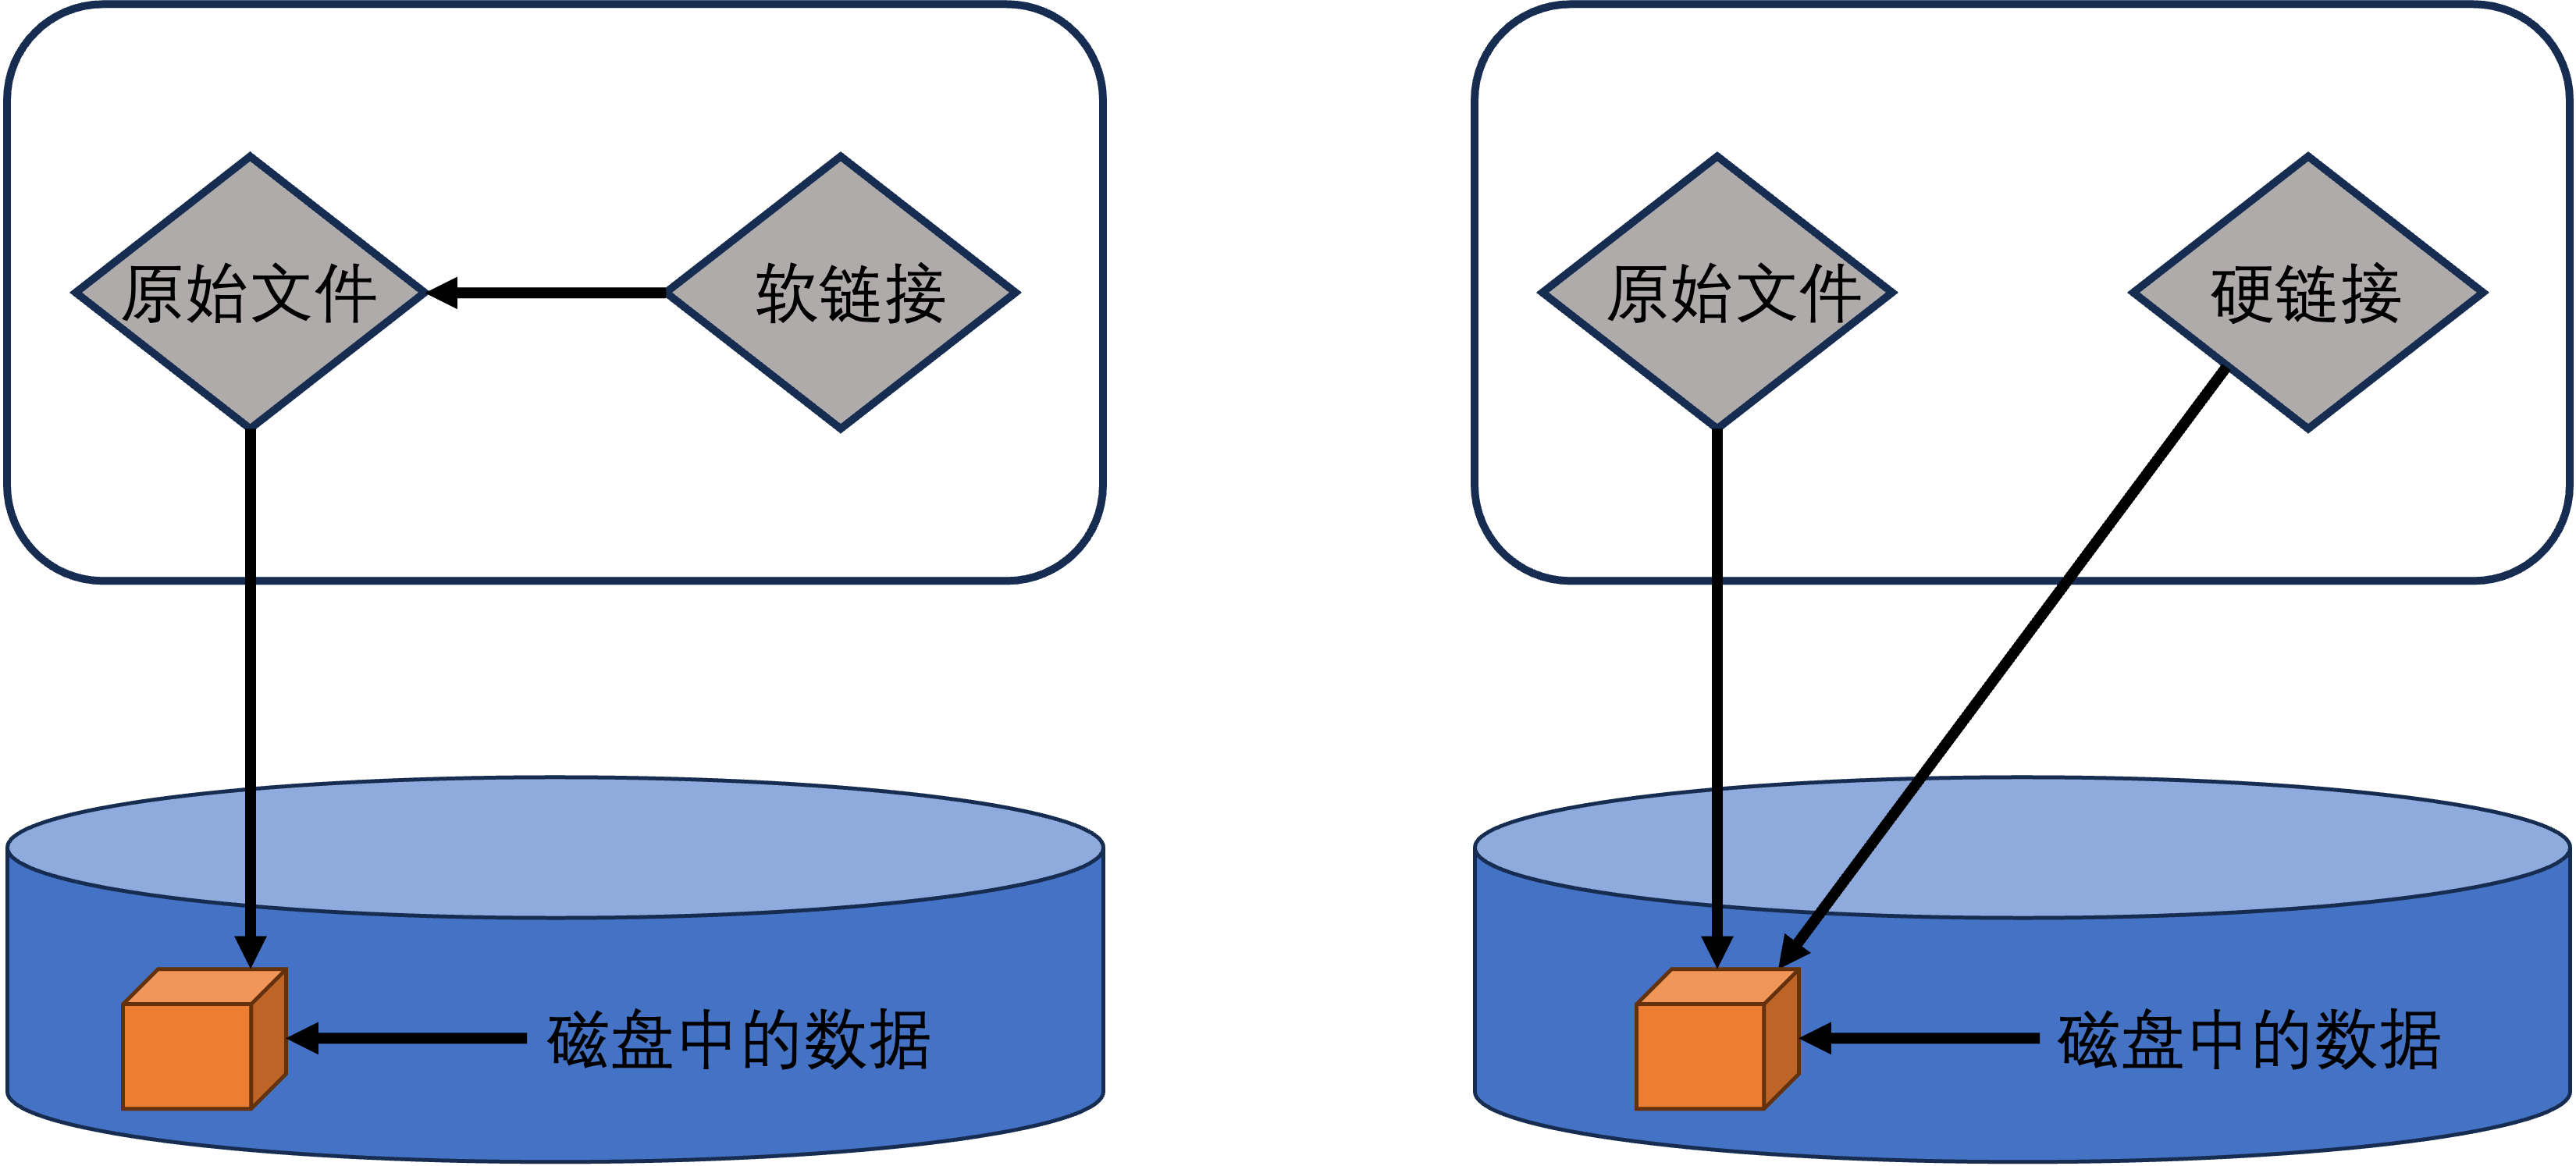
\includegraphics[width=\textwidth]{figures/07-09-软连接与硬连接示意图.png}
    \caption{
        软链接与硬链接示意图
    }
    \label{fig:link}
\end{figure}
\subsection{管道机制}
管道是一种最基本的进程间通信机制,作用于有血缘关系的进程之间,完成数据传递。其本质是一个伪文件,也就是一个小的内核缓冲区,作为一对文件描述符暴露给进程,一个用于读取,一个用于写入。将数据写入管道的一端使得该数据可用于从管道的另一端读取。

与管道相关的系统调用有pipe、write、read等,功能分别为创建、写入、读取管道。后两个系统调用已在其他章节详细解释,在这里着重介绍pipe系统调用。pipe系统调用的定义如下:
\begin{lstlisting}[language=rust]
    sys_pipe2(pipefd: usize, flags: u32) -> isize
\end{lstlisting}

pipeline ()创建一个管道,一个可用于进程间通信的单向数据通道。数组pipefd用于返回两个引用管道末端的文件描述符。pipefd[0]指的是管道的读取端。pipefd[1]指的是管道的写端。写入管道写入端的数据由内核缓冲,直到从管道读取端读取。

flags可以包含如下标志位:

O_CLOEXEC。设置两个读写文件描述符的close-on-exec标志。正常情况下,当一个进程执行一个新的程序时,新程序会继承其父进程的文件描述符。文件描述符是用于访问文件、套接字和其他I/O资源的抽象。O_CLOEXEC标志则用于指定文件描述符在执行新程序时是否应该被关闭。当设置过此标志后,执行一个新程序时,该文件描述符会被自动关闭。也就是说,新程序将不再继承父进程中的这个文件描述符。
              
O_DIRECT。创建一个以“分组”模式进行I/O的管道。对管道的每次write都被视为一个单独的分组,而从管道读取数据时,read系统调用将一次读取一个分组。需要注意的点有:大于PIPE_BUF字节的写操作将被拆分成多个分组。如果read指定的缓冲区大小小于下一个分组的大小,则将读取请求的字节数,并丢弃分组中的多余字节。指定缓冲区大小为PIPE_BUF足以读取可能的最大分组。不支持零长度的分组,read指定缓冲区大小为零的操作是无操作的,并返回0。

O_NONBLOCK。在新文件描述符所引用的打开文件描述符上设置O_NONBLOCK文件状态标志,指示文件描述符应该以非阻塞模式打开。在非阻塞模式下,文件描述符的 I/O 操作不会阻塞(即不会导致调用进程挂起等待),而是会立即返回,无论操作是否完成。这种模式在需要异步操作或需要避免长时间阻塞的场景下非常有用。

当前,在NPUCore中,只支持O_CLOEXEC标志位。

在内核中,pipe的数据结构本质上是一个环形队列,数据从写端流入管道,从读端流出,这样就实现了进程间通信。对应NPUCore的代码如下。队列被初始化为空( head=tail=0),且没有写端的引⽤计数。
\begin{lstlisting}[language=rust]
    impl PipeRingBuffer {
    fn new() -> Self {
        // let mut vec = Vec::<u8>::with_capacity(RING_DEFAULT_BUFFER_SIZE);
        // unsafe {
        //     vec.set_len(RING_DEFAULT_BUFFER_SIZE);
        // }
        Self {
            arr: Box::new([0u8; RING_DEFAULT_BUFFER_SIZE]),
            head: 0,
            tail: 0,
            status: RingBufferStatus::EMPTY,
            write_end: None,
            read_end: None,
        }
    }
}
\end{lstlisting}

初始化这个队列之后,实例化两个 Pipe 两端,并分别定义为写端与读端,也就是设置其对应的标志位:
\begin{lstlisting}[language=rust]
    impl Pipe {
    pub fn read_end_with_buffer(buffer: Arc<Mutex<PipeRingBuffer>>) -> Self {
        Self {
            readable: true,
            writable: false,
            buffer,
        }
    }
    pub fn write_end_with_buffer(buffer: Arc<Mutex<PipeRingBuffer>>) -> Self {
        Self {
            readable: false,
            writable: true,
            buffer,
        }
    }
}
\end{lstlisting}

上述代码已经完成了sys_pipe2系统调用的主体过程。

\begin{figure}[htb]
    \centering
    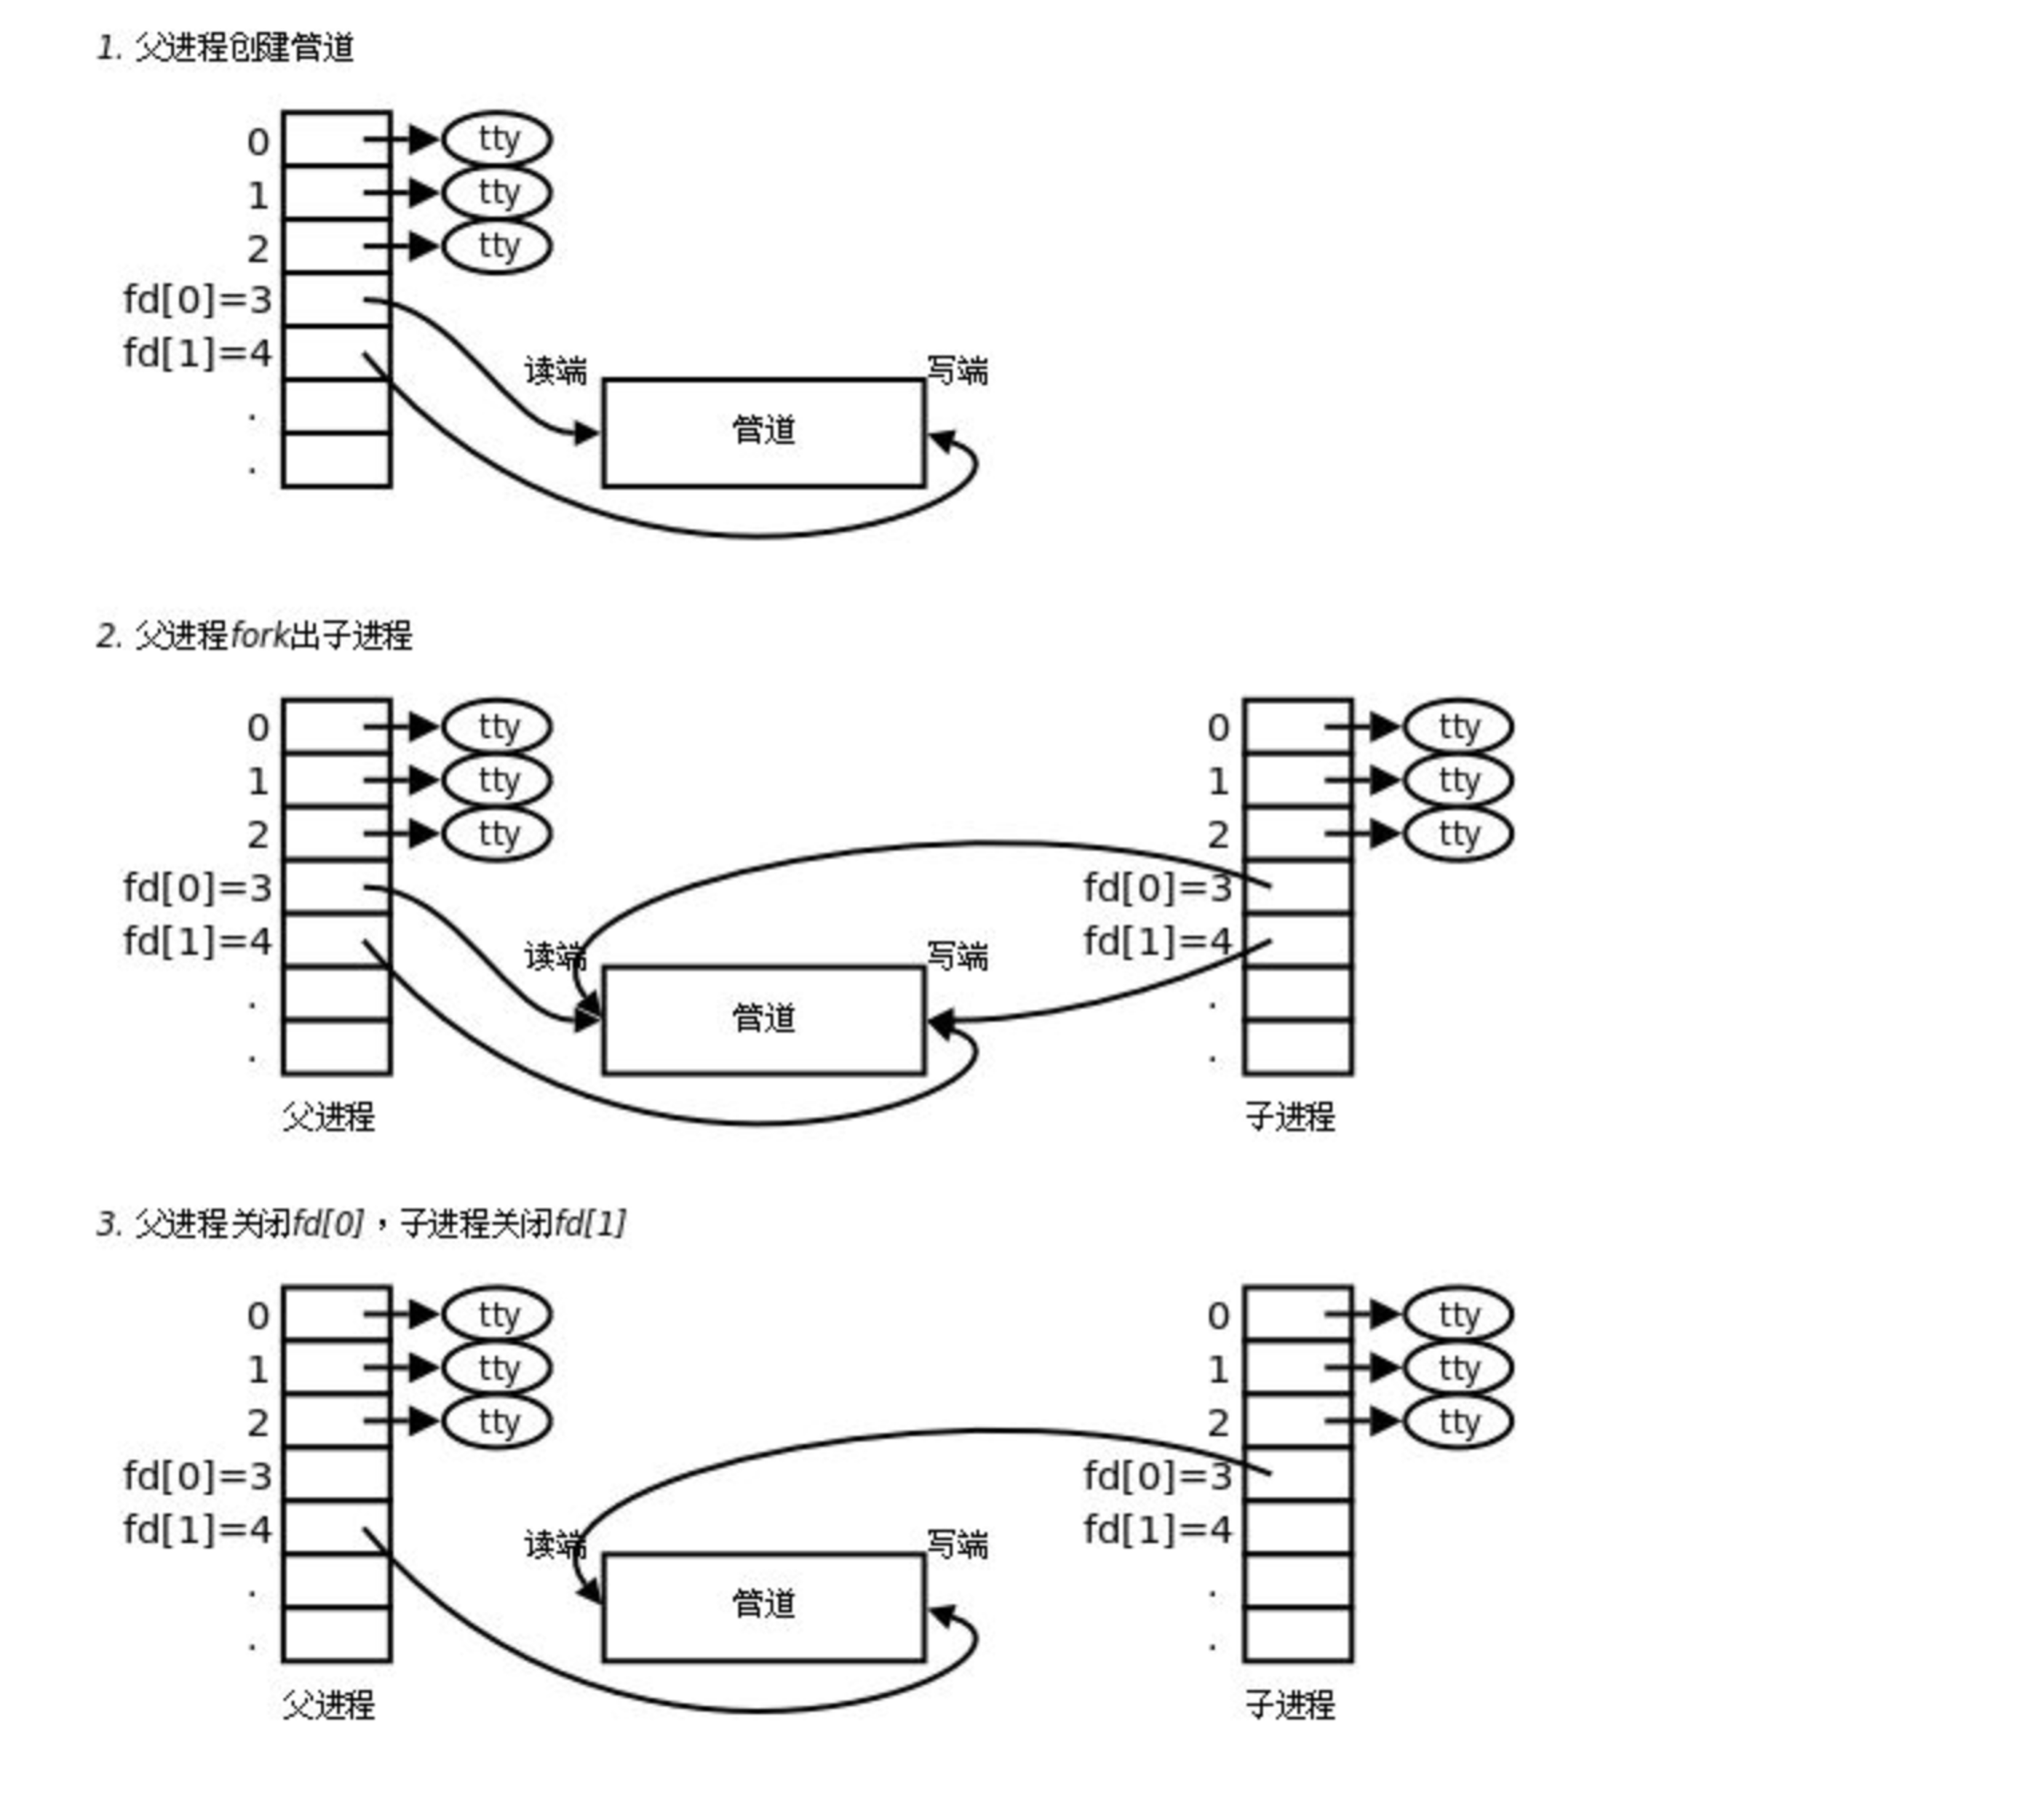
\includegraphics[width=\textwidth]{figures/07-09-管道操作示意图.png}
    \caption{
        管道操作示意图
    }
    \label{fig:pipe}
\end{figure}

下面介绍pipe的使用过程。一般情况下,管道创建成功以后,创建该管道的进程(父进程)同时掌握着管道的读端和写端。要实现父子进程间通信,通常可以采用如\ref{fig:pipe}所示的步骤:

1. 父进程调用pipe系统调用创建管道,得到两个文件描述符pipefd[0]、pipefd[1]指向管道的读端和写端。

2. 父进程调用fork创建子进程,那么子进程也有两个文件描述符指向同一管道。

3. 父进程关闭管道读端,子进程关闭管道写端。父进程可以向管道中写入数据,子进程将管道中的数据读出。

使用管道时,存在以下4种特殊情况(假设都是阻塞I/O操作,没有设置O_NONBLOCK标志):

1. 如果所有指向管道写端的文件描述符都关闭了(管道写端引用计数为0),而仍然有进程从管道的读端读数据,那么管道中剩余的数据都被读取后,再次read会返回0,就像读到文件末尾一样。

2. 如果有指向管道写端的文件描述符没关闭(管道写端引用计数大于0),而持有管道写端的进程也没有向管道中写数据,这时有进程从管道读端读数据,那么管道中剩余的数据都被读取后,再次read会阻塞,直到管道中有数据可读了才读取数据并返回。

3. 如果所有指向管道读端的文件描述符都关闭了(管道读端引用计数为0),这时有进程向管道的写端write,那么该进程会收到信号SIGPIPE,通常会导致进程异常终止。当然也可以对SIGPIPE信号实施捕捉,不终止进程。具体方法信号章节详细介绍。

4. 如果有指向管道读端的文件描述符没关闭(管道读端引用计数大于0),而持有管道读端的进程也没有从管道中读数据,这时有进程向管道写端写数据,那么在管道被写满时再次write会阻塞,直到管道中有空位置了才写入数据并返回。


最后介绍pipe的关闭过程。由于系统调⽤ sys_pipe 为参数 pipe 写⼊了写端和读端两个指向进程控制块的⽂件描述符表的相关位置,通过系统调⽤ sys_close 可以⽤关闭⽂件的相同的⽅式关闭管道的⼆端。sys_close 将⽂件描述符标记为空,会使得对应的 Arc 引⽤被销毁。写端和读端都被关闭后,buffer的引⽤对象,即管道⾃⾝的引⽤计数减少到0,导致管道⾃⾝被销毁,管道也得以关闭。


